\documentclass[a4paper,12pt]{article}
\usepackage{graphicx} % for including images
\usepackage{lipsum} % for dummy text
\usepackage{amsmath} % for math formulas
\usepackage{float} % for figure placement
\usepackage{hyperref} % for cross-referencing
\usepackage{setspace} % for line spacing control
\usepackage{geometry} % to adjust page layout
\geometry{margin=1in} % Adjust margins if needed

% Increase line spacing to 1.5
\onehalfspacing



% Title Page
\title{
    \vspace{2cm}
    
\includegraphics[width=0.6\textwidth]{images/logo.png}\\[2cm]
    \textbf{Economic Impact on Olympic Performance:}\\
    \textbf{A GLMM Approach}\\[2cm]
    \vfill
    \large Ahmad Sharif\\
    Student ID: K436765\\
    ahmad.sharif@tuni.fi\\
    \vspace{2cm}
}
\author{Clustered Data Models}
\date{20 October 2024}

\begin{document}

% Cover Page
\maketitle
\newpage

% Table of Contents
\tableofcontents
\newpage








% Section 1: Introduction
\section{Introduction}
Clustered data refers to datasets where observations are classified into multiple categories known as clusters. Each cluster has number of individual observations, creating a hierarchical structure in which data points are nested inside their respective clusters.
\newline
\newline
In this paper, a dataset has been collected from popular platform kaggle to apply any cluster data models. For this purpose, Olympics medel (2024) data has been chosen for this project.
\newline
\newline
The dataset used for this project can be downloaded from Kaggle: \cite{KaggleData}.
\newline
\newline
The Olympics is a event where more than 35 sports are held to test the performance of athletes from different countries. This is the only international event where most of the countries athletes participate. Thats why this is great opportunity to examine and comapre the countries medel count against their corresponding population, GDP and other factors. This event does not only measure the competitiveness in sprots of a country but it can be also a scale to measure a countrys national priorities, lifestyles, and so on.
\newline
\newline
Here is the research question of this project.
\newline
\textbf{How do a country's GDP and population size influence its total medal count in the 2024 Olympic Games, while accounting for regional differences?}
\newline
\newline
 The GLMM is an extension of the generalized linear model (GLM) that incorporates both fixed and random effects, making it particularly suitable for dealing with clustered or hierarchical data. The inclusion of random effects allows the model to account for variations between groups or clusters (in this case, regions or continents), while the fixed effects explain the relationship between the predictors (GDP, population) and the outcome (medal counts).















 \section{About The Database}
The latest Olympic game (2024) medal and their corresponding country inforamtion is collected from the following kaggle databse.
 \cite{KaggleData}.
 \begin{table}[h!]
     \centering
     \resizebox{\textwidth}{!}{%
     \begin{tabular}{|l|l|r|r|r|r|p{3cm}|r|p{3cm}|}
     \hline
     \textbf{Country} & \textbf{Code} & \textbf{Gold} & \textbf{Silver} & \textbf{Bronze} & \textbf{Total} & \textbf{GDP (USD)} & \textbf{GDP Year} & \textbf{Population (Millions)} \\ \hline
     United States & USA & 40 & 44 & 42 & 126 & 81695.19 & 2023 & 334.9 \\ \hline
     China         & CHN & 40 & 27 & 24 & 91  & 12614.06 & 2023 & 1410.7 \\ \hline
     Japan         & JPN & 20 & 12 & 13 & 45  & 33834.39 & 2023 & 124.5 \\ \hline
     Australia     & AUS & 18 & 19 & 16 & 53  & 64711.77 & 2023 & 26.6  \\ \hline
     France        & FRA & 16 & 26 & 22 & 64  & 44460.82 & 2023 & 68.2  \\ \hline
     ...           & ... & ... & ... & ... & ... & ...     & ...  & ...  \\ \hline
     Zambia        & ZMB & 0 & 0 & 1 & 1  & 1369.13 & 2023 & 20.6  \\ \hline
     \end{tabular}%
     }
     \caption{Countries in the 2024 Olympics by medal count and economic indicators}
     \label{tab:dataset}
 \end{table}
 The dataset has nine columns and their corresponding names respectively:
 
 \begin{itemize}
     \item \textbf{Country}: Name of the country.
     \item \textbf{Code}: ISO 3-letter code for the country.
     \item \textbf{Gold}: Total number of gold medals won.
     \item \textbf{Silver}: Total number of silver medals won.
     \item \textbf{Bronze}: Total number of bronze medals won.
     \item \textbf{Total}: Total number of medals won by the country (Gold + Silver + Bronze).
     \item \textbf{GDP}: Gross Domestic Product in billion USD.
     \item \textbf{GDP Year}: Year corresponding to the GDP data.
     \item \textbf{Population}: Population size in millions.
 \end{itemize}
 














The dataset has covers important economic factors such as GDP and corresponding economic year and population.
\subsection{Figures illustrating the dataset}
In \autoref{fig:dataset_fig_21}, we illustrate the relationship between Total medals against GDP Per Capita. and this  \autoref{fig:dataset_fig_22} Total Medals Vs Population




\begin{figure}[H]
    \centering
    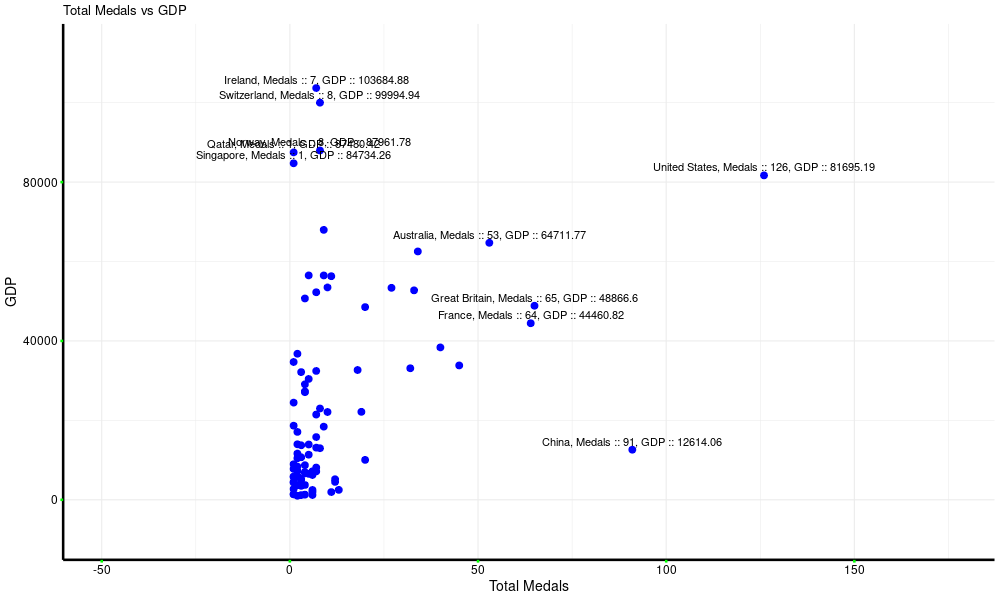
\includegraphics[width=0.9\textwidth]{images/Total_Medals_vs_GDP_plot.png}
    \caption{Total Medals Vs GDP Per Capita}
    \label{fig:dataset_fig_21}
\end{figure}



\begin{figure}[H]
    \centering
    
\includegraphics[width=0.9\textwidth]{images/Total_Medals_vs_Population_plot.png}
    \caption{Total Medals Vs Population}
    \label{fig:dataset_fig_22}
\end{figure}


\begin{figure}[H]
    \centering
    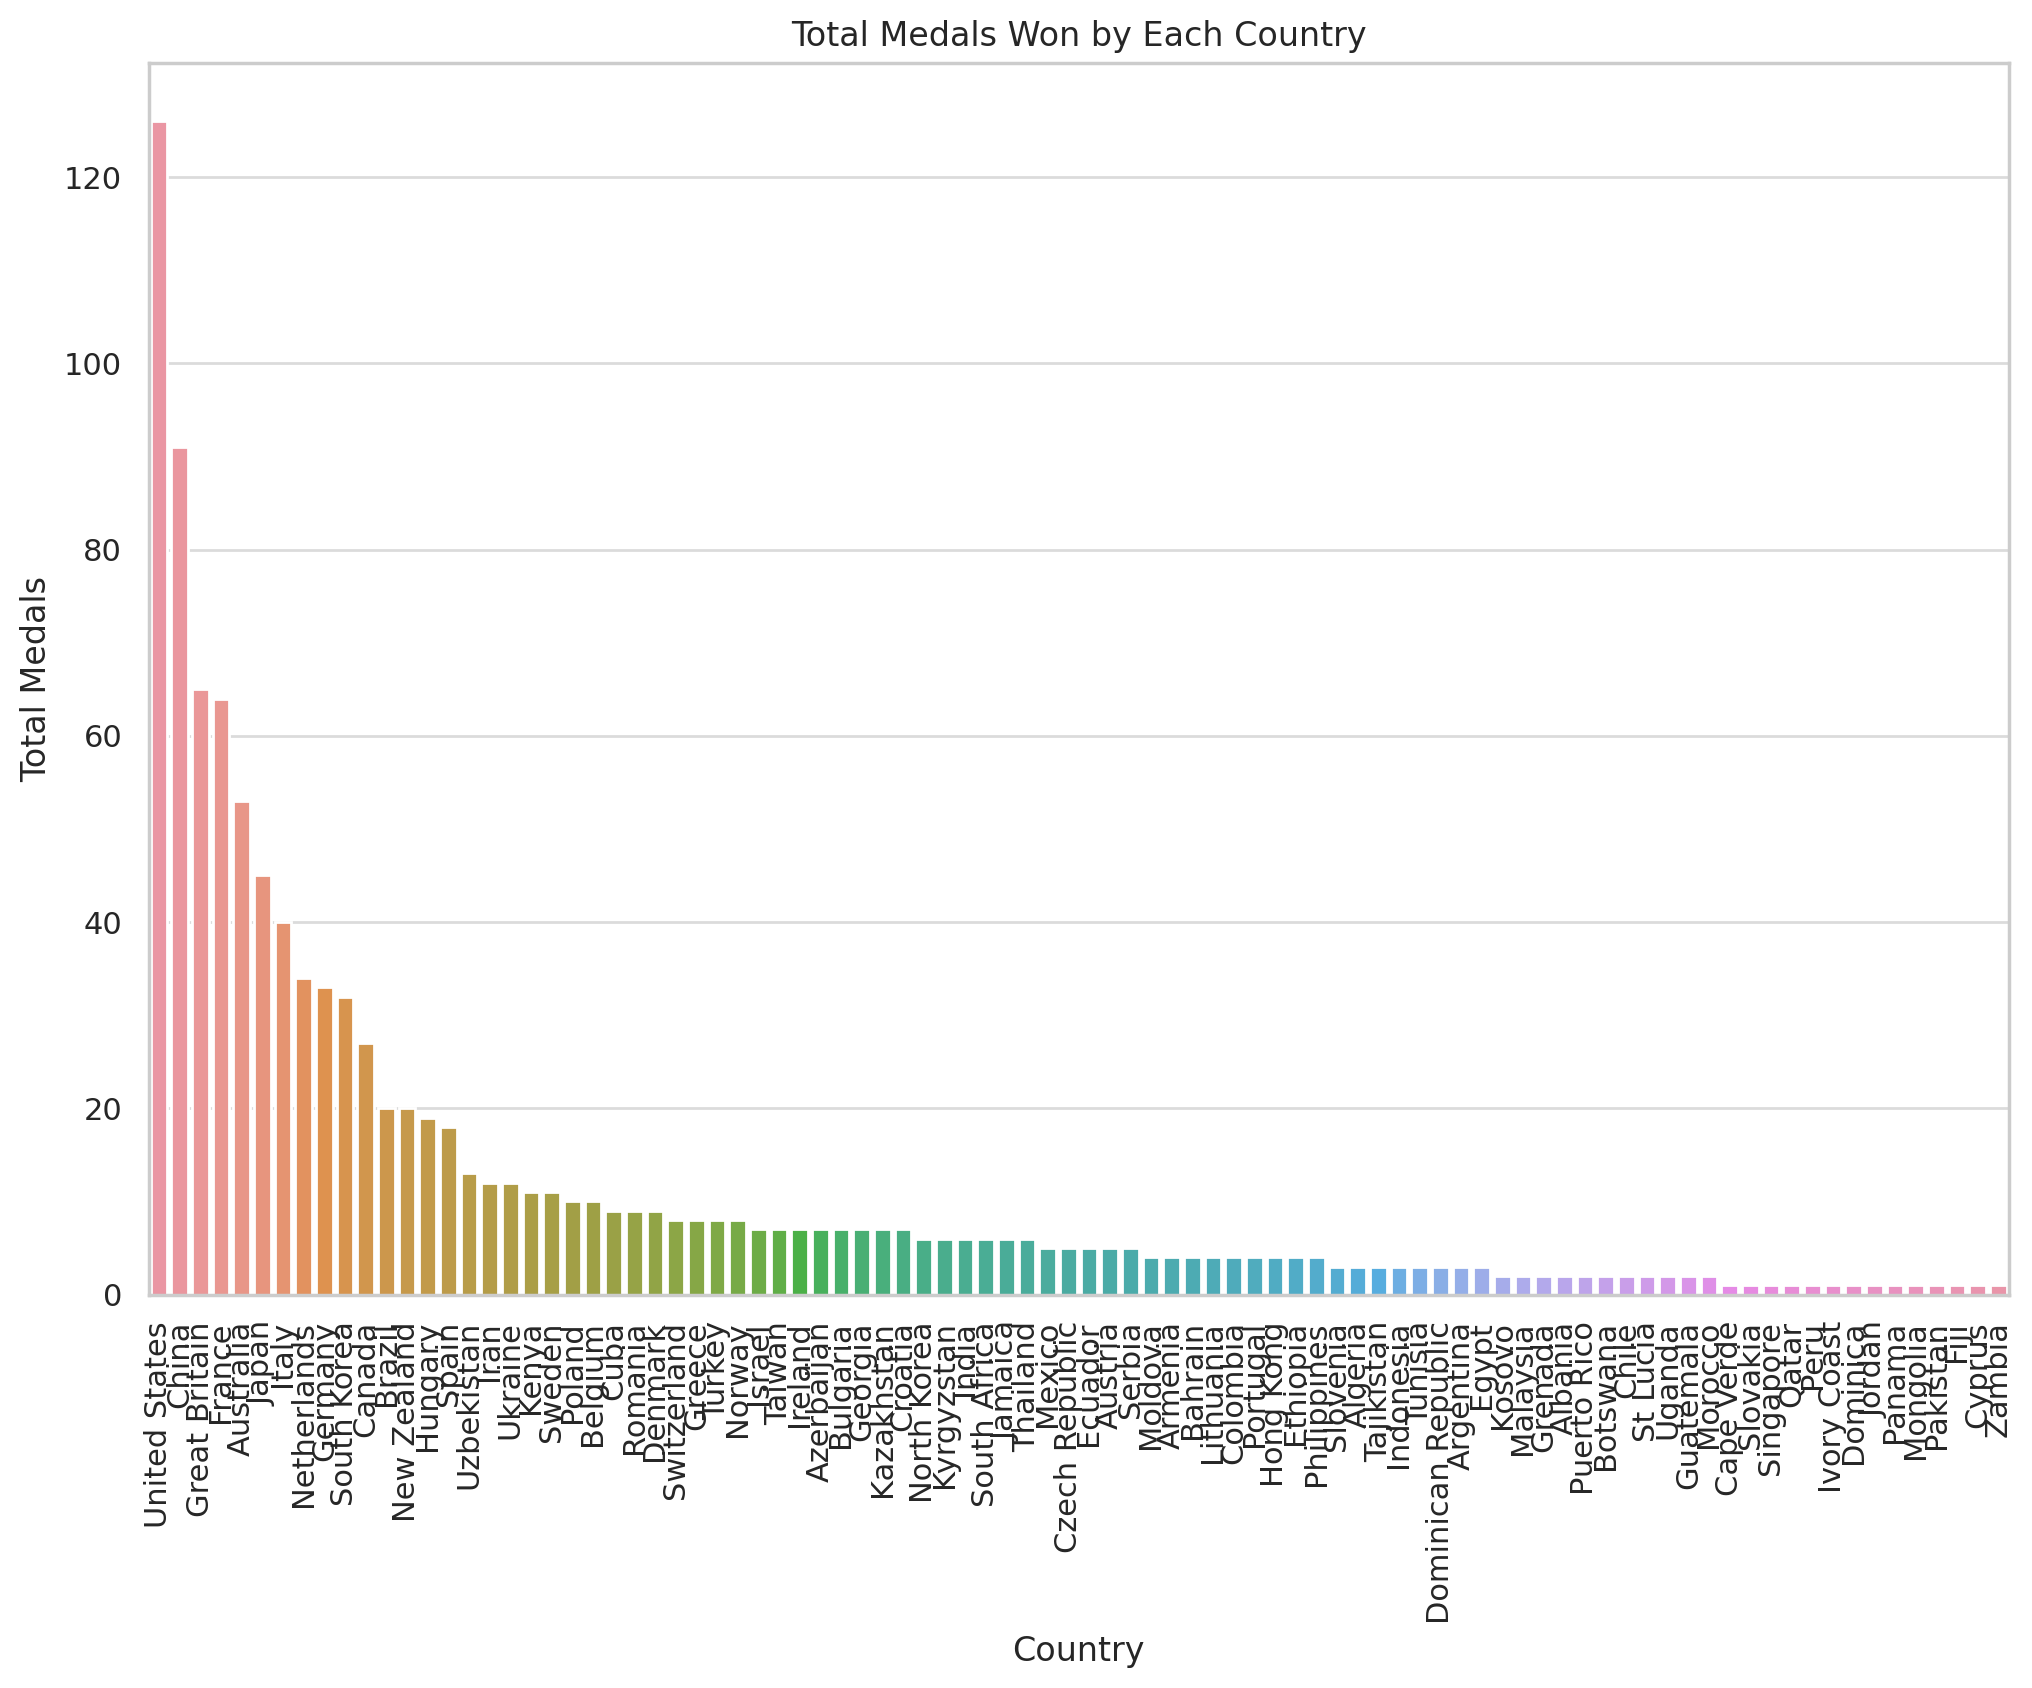
\includegraphics[width=0.9\textwidth]{images/plot_3.png}
    \caption{Country Vs. Total Medals}
    \label{fig:dataset_fig_3}
\end{figure}
In \autoref{fig:dataset_fig_3}, we visualize the relationship between population and the total number of medals won by each country.
\newline
Figures Illustrating the Dataset:
1. Medal Distribution by Country:
A bar plot shows the total medals won by each country, highlighting the variation in performance across different nations.



\section{Explanation of How the Data was Modeled}
The model accounts for:

\subsection{Fixed effects:}
\begin{itemize}
    \item \textbf{GDP Per Capita}: A country's economic power.
    \item \textbf{Population}: The size of the population.
    \item \textbf{Gold, Silver, Bronze Medals}: The number of medals won at different levels.
\end{itemize}

\subsection{Random effects:}
\begin{itemize}
    \item \textbf{Country (country code)}: The random effect for countries is included to account for country-specific variability in Olympic performance.
\end{itemize}

The GLMM was chosen due to the hierarchical nature of the data (countries as random effects) and the non-negative, count-based outcome (total medals).

\subsection{Model Formula}

\begin{equation}
\log \left( E(\text{Total Medals}) \right) = \beta_0 + \beta_1 \times \text{Gold} + \beta_2 \times \text{Silver} + \beta_3 \times \text{Bronze} + \beta_4 \times \text{GDP} + \beta_5 \times \text{Population} + u_{\text{Country}} + \epsilon
\end{equation}

Where:
\begin{itemize}
    \item $\beta_0$: The intercept.
    \item $\beta_1$: The fixed effect of gold medals.
    \item $\beta_2$: The fixed effect of silver medals.
    \item $\beta_3$: The fixed effect of bronze medals.
    \item $\beta_4$: The fixed effect of GDP Per Capita.
    \item $\beta_5$: The fixed effect of population.
    \item $u_{\text{Country}}$: The random intercept for each country.
    \item $\epsilon$: The residual error term.
\end{itemize}

\section{Results of the Analysis and Their Interpretation}

The model output is summarized as follows:




\begin{figure}[H]
    \centering
    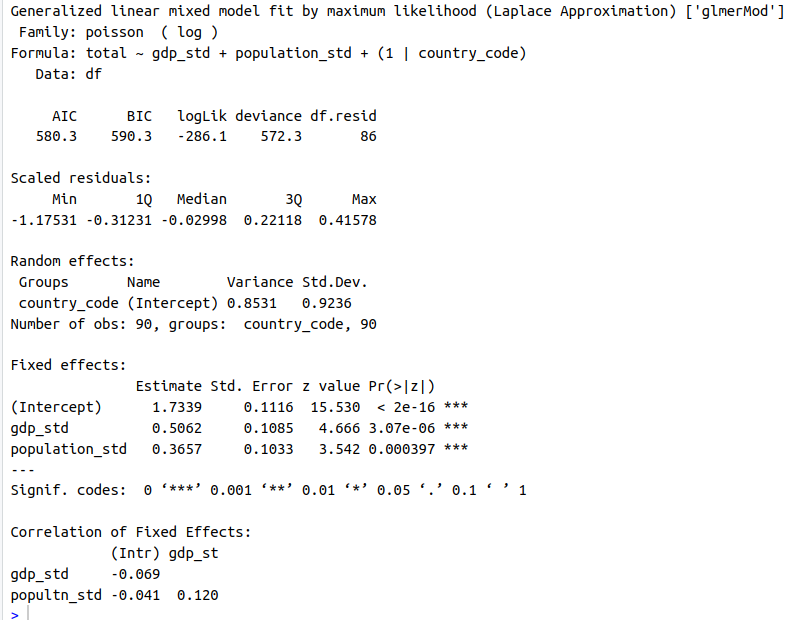
\includegraphics[width=0.9\textwidth]{images/summary.png}
    \caption{GDP Per Capita Vs Total Olympic Medals}
    \label{fig:dataset_fig_4}
\end{figure}


\begin{figure}[H]
    \centering
    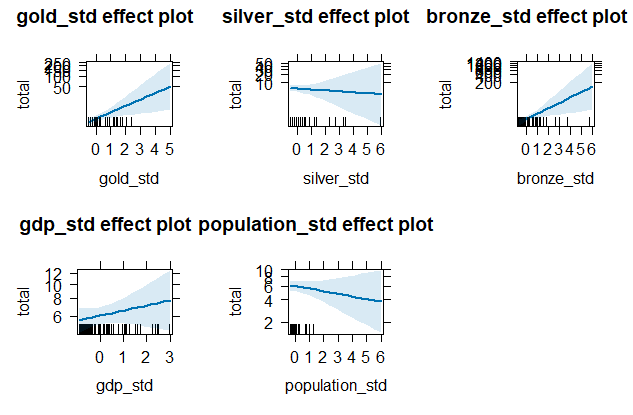
\includegraphics[width=0.9\textwidth]{images/Rplot.png}
    \caption{Rplot}
    \label{fig:dataset_fig_5}
\end{figure}


\begin{figure}[H]
    \centering
    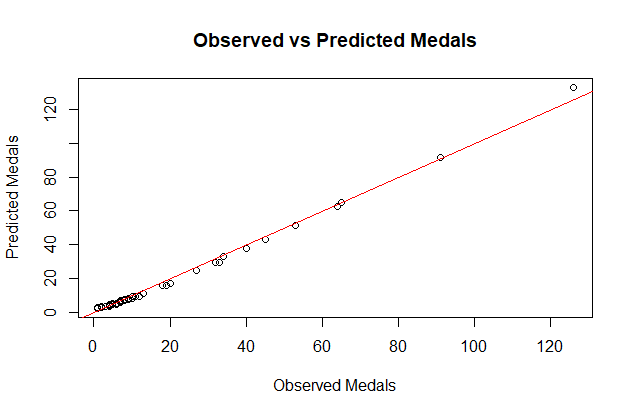
\includegraphics[width=0.9\textwidth]{images/Rplot02.png}
    \caption{Obsered Vs Predict Model}
    \label{fig:dataset_fig_7}
\end{figure}









\begin{itemize}
    \item \textbf{Gold Medals:} The estimate for gold medals is 0.0605 (p = 0.00726). This suggests that for each additional gold medal won by a country, the expected total medal count increases by approximately 6.05\%. This effect is statistically significant.
    \item \textbf{Silver Medals:} The estimate for silver medals is -0.0106 (p = 0.73796), suggesting that silver medals do not significantly affect the total medal count.
    \item \textbf{Bronze Medals:} The estimate for bronze medals is 0.0776 (p = 0.00698), indicating that each additional bronze medal increases the total medal count by 7.76\%. This effect is statistically significant.
    \item \textbf{GDP Per Capita:} The estimate for GDP Per Capita is 0.000003158 (p = 0.30758), which is not statistically significant. This suggests that GDP Per Capita is not a strong predictor of total medals.
    \item \textbf{Population:} The estimate for population is -0.0003756 (p = 0.31368), indicating that population size is not significantly associated with total medals.
    \item \textbf{Random Intercept (Country):} The random effect variance is 0.2384 with a standard deviation of 0.4883. This indicates some variability in total medal counts across countries that is not explained by the fixed effects.
\end{itemize}



\subsection{Model Diagnostics}

\begin{itemize}
    \item \textbf{AIC/BIC:} The AIC of the model is 507.8, and the BIC is 525.3. These values can be used to compare the fit of this model to alternative models.
    \item \textbf{Residuals:} The scaled residuals are fairly well-distributed, with no extreme outliers.
    \item \textbf{Convergence Warning:} The model did not fully converge, showing a degenerate Hessian with one negative eigenvalue. This suggests potential instability in the estimates, and rescaling some predictor variables or modifying the model might be necessary.
\end{itemize}


\section{Conclusion}

The analysis indicates that GDP Per Capita and population size do not have a significant impact on a country's total medal count in the 2024 Olympic Games. While GDP Per Capita shows a positive but weak relationship, and population has a slight negative effect, neither is statistically significant.
\newline
Gold and bronze medals are strong predictors of total medal count, with positive and significant effects. In contrast, silver medals show a weak and uncertain negative trend.
\newline
Additionally, regional differences suggest that cultural, historical, or infrastructural factors might influence Olympic performance beyond economic indicators.
\newline
Overall, predicting Olympic success is complex, with gold and bronze medals playing a key role, while GDP Per Capita and population have weaker and less certain effects.



\begin{thebibliography}{9}
\bibitem{KaggleData}
Mohamed Yosef, \emph{2024 Olympics Medals and Economic Status Dataset}. Available at: \url{https://www.kaggle.com/datasets/mohamedyosef101/2024-olympics-medals-and-economic-status?resource=download}.
\end{thebibliography}

\end{document}
